\documentclass{mycv}

%\newcommand{\CVRole}{Entwicklungsingenieur}
%\newcommand{\CVFields}{autonomes Fahren, Fahrzeugdynamik und Softwareentwicklung}

\newcommand{\CVRole}{software architecht}
\newcommand{\CVFields}{autonomous driving, machine learning and artificial
intelligence}


\begin{document}
\sloppy % this restricts words spilling out of the margins
\color{templateColor1}
\pagenumbering{gobble}
\AddToShipoutPicture{\BackgroundPic}

\normalfont
\begin{minipage}[c]{0.3\textwidth}
	\centering
	%\includegraphics[width=4.5cm,height=6cm]{example-image-a}
	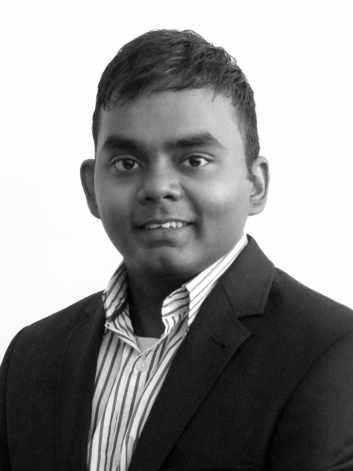
\includegraphics[width=4.5cm,height=6cm]{../img/CV_Photo.jpg}
\end{minipage}
\begin{minipage}[]{0.7\textwidth}

  \vspace{5mm}
	{\Huge CHANDRAMOULI}\\

	{\Huge GNANASAMBANDHAM}
	\vspace{2mm}

	%{\large SIMULATION ENGINEER}
	\vspace{2mm}

  Bromenlandweg 10\\
	71034 B{\"o}blingen\\

	\telephoneIcon 0179 658 8043\\
	\mailIcon \href{mailto:chandramouli681990@gmail.com}{chandramouli681990@gmail.com}
  
  \vspace{13mm}
\end{minipage}

{\rlap{\color{templateColor1}\rule[0mm]{\textwidth}{\ulinewidth}}}
\columnratio{0.39}
\setlength{\columnsep}{2.5em}
\setlength{\columnseprule}{\ulinewidth}
\colseprulecolor{templateColor1}
\begin{paracol}{2}
		%\lsection{ANGESTREBTE STELLE}
		% Deutsch #################################################################

		%Ich bin ein leidenschaftlich \,neugieriger
		%Ingenieur mit exzellenten interkulturellen Kommunikationsfähigkeiten. Ich
		%habe 6 Zeitschriftartikel in renommierten Fachzeitschriften publiziert
		%und an mehreren erfolgreichen DFG-Forschungsantr{\"a}gen entscheidend
		%mitgewirkt. All dies war möglich, dank meiner sehr guten
		%Anpassungsf{\"a}higkeit an schnell wechselnden Umgebungen und meiner
		%hervorragenden analytischen, Projektmanagement- und Team-F{\"a}higkeiten,
		%die ich an der Universität erworben habe. Ich suche eine T{\"a}tigkeit als
		%\CVRole, idealerweise im Bereich \CVFields.\\

		% English #################################################################

		\lsection{PROFILE}
		I am an passionately curious engineer with excellent intercultural
		communication skills. I have been first author of 6 peer-reviewed journal
		articles and have played a crucial role in several successful research
		proposals funded by the German Research Foundation (DFG). All this was
		possible, thanks to my exceptional adaptability to new/rapidly changing
		environments and my extraordinary analytical, project management and team
		working skills gained through my time at the academia.  I am looking for a
		challenging oportunity as a \CVRole, prefarrably in the field of
		\CVFields.\\

	  \lsection{LANGUAGES}
	  \begin{doublespace}
			\begin{tabular}{%
				p{2cm}%
				>{\raggedleft\arraybackslash}p{4.5cm}}
			{\mybox\mybox\mybox\mybox\mybox}  &
			{Proficient | German} \\
      {\mybox\mybox\mybox\mybox\mybox} & 
			{Proficient | English}\\
      {\mybox\mybox\mybox\mybox\mybox}  & 
      {Mother tounge | Tamil}  \\
      {\mybox\mybox\mybox\mybox\myboxo}  & 
      {Advanced | Hindi}\\\\
		\end{tabular}
	  \end{doublespace}

		\lsection{WEB}
		%\begin{tabular}{ll}
		%\githubIcon & {\bfseries GITHUB}\\{\footnotesize
		%	https://github.com/chandramouli6890} 
		%\end{tabular}
		\begin{minipage}[c]{0.31\textwidth}
			\begin{flushright}
				{\bfseries GITHUB}\\
				{\footnotesize
					\href{https://github.com/chandramouli6890}{\link{https://github.com/chandramouli6890}}}
			\end{flushright}
		\end{minipage}
		\begin{minipage}{0.05\textwidth}
			\githubIcon
		\end{minipage}
		\vspace{3mm}

		\begin{minipage}[c]{0.31\textwidth}
			\begin{flushright}
				{\bfseries Linkedin}\\
				{\footnotesize
					\href{https://linkedin.com/in/gnanasambandhamc}{\link{https://linkedin.com/in/gnanasambandhamc}}}
			\end{flushright}
		\end{minipage}
		\begin{minipage}{0.05\textwidth}
			\linkedinIcon
		\end{minipage}
		\vspace{3mm}

		\begin{minipage}[c]{0.31\textwidth}
			\begin{flushright}
				{\bfseries Medium}\\
				{\footnotesize \href{https://chandramoulig.medium.com}{\link{https://chandramoulig.medium.com}}}
			\end{flushright}
		\end{minipage}
		\begin{minipage}{0.05\textwidth}
			\mediumIcon
		\end{minipage}
		\vspace{3mm}

		\begin{minipage}[c]{0.31\textwidth}
			\begin{flushright}
				{\bfseries Matlab}\\
				{\footnotesize
					\href{https://de.mathworks.com/matlabcentral/profile/authors/4267772}{\link{MatlabCentral	Profil}}}
			\end{flushright}
		\end{minipage}
		\begin{minipage}{0.05\textwidth}
			\matlabIcon
		\end{minipage}


		%\lsection{KERNKOMPETENZEN}
		%\begin{minipage}[c]{0.4\textwidth}
		%	\begin{tikzpicture}[overlay]
		%		\begin{scope}[shift={(3.7,2.9)}]
    %      \pie[
    %          color = {
    %              templateColor1,
    %              templateColor2,
    %              templateColor3,
    %              templateColor4,
    %              templateColor5},
    %          hide number,
		%      		radius=1.5,
		%      		before number=\phantom,
		%      		after number=
    %      ]
		%      {20/, 20/, 10/, 10/, 40/}
		%			\draw[templateColor1,fill=white] (0,0) circle (1.0); further text
		%			\draw[templateColor1,very thin] ( 0.8,-1  ) -- (1.2,-1.2 ) -- (1.4,-1.5 );
		%			\draw[templateColor1,very thin] (-1.2,-0.5) -- (-1.6,-0.8) -- (-1.6,-1.5);
		%			\draw[templateColor1,very thin] (-1.2, 0.5) -- (-1.6, 0.8) -- (-1.6, 1.5);
		%			\draw[templateColor1,very thin] ( 1.2, 0.8) -- ( 1.6, 1.0) -- ( 1.6, 1.5);
		%			\draw[templateColor1,very thin] ( 0.0, 1.2) -- ( 0.0, 2.0);
		%\end{scope}
		%\end{tikzpicture}
		%	\begin{picture}(100,160)
		%		%\put(20,40){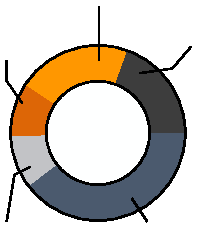
\includegraphics{pie_chart_core_competency.pdf}}
		%		\put(110,25){\parbox{2.2cm}{\centering Software\-entwicklung}}
		%		\put(30,25){\parbox{2.2cm}{\centering{Projekt\-management}}}
		%		\put(30,130){Sprachen}
		%		\put(70,150){\parbox{2.2cm}{\centering analytisches Denken}}
		%		\put(130,130){Forschung}
		%	\end{picture}
		%\end{minipage}
		%\includegraphics[width=5cm]{example-image-a}
		%\begin{minipage}[c]{0.3\textwidth}
		%	\begin{picture}(100,160)
		%		%\put(20,40){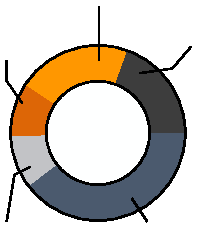
\includegraphics{pie_chart_core_competency.pdf}}
		%		\put(80,25){\parbox{2.2cm}{\centering Software\-entwicklung}}
		%		\put(0,25){\parbox{2.2cm}{\centering{Projekt\-management}}}
		%		\put(0,130){\parbox{2.2cm}{\centering analytisches Denken}}
		%		\put(55,150){Kreativi{\"a}t}
		%		\put(100,130){Forschung}
		%	\end{picture}
		%\end{minipage}
		%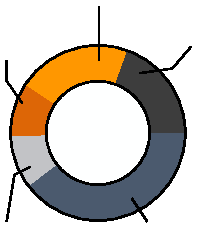
\includegraphics{pie_chart_core_competency.pdf}


\switchcolumn
		\rsection{TECHNICAL SKILLS}
		%\begin{singlespace}
		\begin{doublespace}
		%\begin{onehalfspace}
			\begin{tabular}{p{5cm}!{\color{templateColor1}\vrule}p{6.5cm}}
			{\bfseries Programming Languages: } & {\bfseries Betriebssystem}\\
			{\mybox\mybox\mybox\mybox\mybox 8 years | C/C++}  &
			{\mybox\mybox\mybox\mybox\mybox Linux (Debian, Ubuntu)}\\
      {\mybox\mybox\mybox\mybox\mybox 8 years | Matlab} & 
			{\mybox\mybox\mybox\mybox\myboxo Microsoft Windows}\\
      {\mybox\mybox\mybox\mybox\myboxo 5 years | BASH}  & \\
      {\mybox\mybox\mybox\myboxo\myboxo 3 years | Python}  & \\
		\end{tabular}\vspace{4mm}
		\end{doublespace}
		%\end{singlespace}

	 {\bfseries Software Skills:}
	 \begin{itemize}
		 \item {\bfseries Matlab/Simulink:} Modelling, \,simulation,
			 numerical optimization, C/C++ MEX API, SiL/HiL simulations
		 \item {\bfseries Python:} Flask, NumPy, SciPy, Pandas
		 \item{\bfseries Multibody-Simulation:}  LMS Virtual.Lab Motion, Neweul-M$^2$, 
			 MSC Adams, Project Chrono
		 %\item {\bfseries Partikelsimulation:} Pasimodo, Project Chrono, DualSPHysics
		 \item {\bfseries Data Visualization:} Paraview, PlotlyDash, Matplotlib, Matlab 
		 \item {\bfseries Other Software:}  COMSOL
			 Multiphysics, OpenSCAD, \,Blender \,with Python scripting, OptiSlang
		 %\item {\bfseries Sonstiges:} \LaTeX{}, TikZ, Inkscape, MS Office
	 \end{itemize}\par

	 {\bfseries Software Development Tools:}\par
	 \begin{itemize}
		 \item {\bfseries Technologies:} CUDA GPU Programming, PETSc, EIGEN,
			 Object Oriented Programing (OOP), OpenGL\par
		 \item {\bfseries Version control:} Gitlab, Github, Gitflow
			 Branching-Model\par
		 \item {\bfseries Development Environments:} \verb|vim|, Visual-Studio Code,
			 Eclipse \par
		 \item {\bfseries Debuggers/Profilers:} \verb|gdb|, \verb|valgrind|, \verb|calgrind|,
			 Intel VTune\\
	 \end{itemize}


		
\rsection{PROFESSIONAL CAREER}
%\rsection{BERUFLICHER WERDEGANG}
\subsection{April 2021}{Submission of the doctoral thesis}{Particle Dampers-
Enhancing Energy Dissipation using Fluid/Solid Interactions and Rigid
Obstacle-Grids}
	  \begin{itemize}
			\item Tentative date of the PhD thesis defence:
				{\bfseries 13.07.2021}
		\end{itemize}
		\flushpage
\end{paracol}

{\rlap{\color{templateColor1}\rule[0mm]{\textwidth}{\ulinewidth}}}
%\setlength{\columnseprule}{\ulinewidth}
%\colseprulecolor{templateColor1}
\begin{paracol}{2}
	  \lsection{AWARDS}
	  {\RaggedLeft \bfseries Best Presentation Award\\}
	  {Title}: Optimization of Vehicle Parameters based on Lap-Time
	  Simulations using Multiobjective Evolutionary Algorithm\\\\
	  {\footnotesize This award was offered by ALTEN GmbH in the year 2015 and
			was endowed with {\bfseries500\,\euro{}}.}\\

	  {\RaggedLeft \bfseries Best Presentation Award\\}
	  {Title}: An Adaptive Approach to Real-Time Estimation of
	  Vehicle Dynamics Parameters using Kalman Filtering\\\\
	  {\footnotesize This award was offered by ALTEN GmbH in the year 2014 and
			was endowed with {\bfseries500\,\euro{}}.}\\


	\lsection{SONSTIGE PROJEKTE}
	{\RaggedLeft Juni 2014\\ \bfseries Driver-in-the-Loop Simulator\\}
	As part of my work for the KaRaT Formula Student racing team, I
	have developed a driver-in-the-loop simulator based on a communication
	interface between {IPG CarMaker} and {Matlab/Simulink}.\\

	{\RaggedLeft Juni 2015\\ \bfseries Machine Learning Suite\\}
	Implementation of a Deep Convolution Neural Network (Deep ConvNet) for
	optical character recognition as part of a freelance software project. To
	increase performance the {Matlab MEX API} was used.\\

	{\RaggedLeft Juli 2020\\ \bfseries Raspberry Pi NAS\\}
	As part of a hobby project I had built a versatile Raspberry-Pi home network
	storage (NAS) device with multiple functions, for e.g.\,remote-ssh-access
	over the internet, automatic backups using \verb|rsync|, DNS-server with
	integrated Pi-Hole ad-blocker and HomeBridge server for controlling IOT
	devices using siri.

\switchcolumn
\rsection{PROFESSIONAL CAREER (CONTINUED)}%

\subsection{May 2016 - April 2021}{University of
Stuttgart}{Scientific staff member at the Institute for Engineering and
	Computational Mechanics (ITM)}
	  \begin{itemize}
			\item  Main research areas: 
				\begin{itemize}
					\item Modelling and simulation of particle dampers with
						meshfree Lagrangian methods
			    \item Systematic investigation of underlying dissipation mechanisms in
						particle dampers  
					%\item Untersuchung des Einflusses von einer komplex gestalteten
			    %	PD-Hindernisstruktur sowie die Wirkung von im PD zus{\"a}tzlich
			    %	eingebrachter Fl{\"u}ssigkeit auf die Energiedissipation
			    %\item Steigerung der Energiedissipation in PD durch
			    %	Fluid/Festk{\"o}rper-Interaktion und starren Hindernis-Gittern 
			    %\item Analyse der Merhfrequez	D{\"a}pfungseingenschaften von PD
		\end{itemize}
			\item Planning and execution of measurement campagins of
				vibrating structures using the priniciples of experimental modal analysis
				and laser doppler vibrometry
			\item Development und administration of the particle simulation package 
			{\bfseries \,Pasimodo} in {\bfseries C++}:
			\begin{itemize}
				\item Developent and implementation of efficient algorithms to adequately
					predict the dynamics of fluid-solid systems
				%\item Implementierung des $k$-$\epsilon$ Turbulenzmodells zur
				%	genauere Modellierung der Fluidstr{\"o}mungen
				%\item Koordination von L{\"o}sungen im Falle von Codekonflikten 
				\item Administration of bug-reports und merge-requests in
					\href{https://about.gitlab.com/}{\link{Gitlab}}
				\item Maintaining and developing of the nightly Build-System using
					the principles of continuous integration (CI)
				\item Maintaining the distributed {\bfseries C++} compilation
					system using \href{https://github.com/distcc/distcc}{\link{distcc}}
				\item Administration and development of software releases at \,regular
					intervals using the
					\href{https://nvie.com/posts/a-successful-git-branching-model/}{\link{Gitflow}}
					Branching-Model
				%\item Support f{\"u}r Anwender
			\end{itemize}
			%\item Bearbeitung des Teilprojektes f{\"u}r die Deutsche
			%	Froschungsgemeinschaft (DFG) im Rahmens des Schwerpunkt Programms
			%	\href{https://www.itm.uni-stuttgart.de/spp_1897/projekte2/eberhard/}{\link{SPP
			%	1897 ``Calm, Smooth, Smart''}} zur Modellierung und
			%	Simulation von PD
			%\item Anfertigen von Ver{\"o}ffentlichungen f{\"u}r 
			%	wissenschaftliche Fachzeitschriften und Vortr{\"a}gen auf
			%	internationalen Fachkonferenzen
			%\item Vorbereiten von Forschungsantr{\"a}gen f{\"u}r die DFG 
			\item Teaching activities:
				\begin{itemize}
					\item Organisation und assitance for the lecture ``Ground Vehicle
						Dynamics''
					\item Execution of lab workshops for B.Sc.\,and M.Sc.\,students
					\item Supervision of Bachelor- and Master-Thesis students\\
				\end{itemize}
		\end{itemize}

\subsection{October 2015 - April 2016}{Fraunhofer Institute of Industrial
	Mathematics (ITWM), \quad\quad Kaiserslautern}
{Student Employment}
%{Werkstudentent{\"a}tigkeit in der Abteilung Mathematische Methoden f{\"u}r Dynamik und
%Festigkeit}
	  \begin{itemize}
			\item Implementaion of a POD based model order reduction method for
				high-dimensional nonlinear finite element systems\\
			%\item Entwicklung eines Proper Orthogonal Decomposition basierenden
			%	Verfahrens zur Reduktion von hochdimensionalen nichtlinearen
			%	FE Systemen 
			%\item Implimentierung einer Schnittstelle zwischen {\bfseries Matlab} und
			%FE Programm {\bfseries COMSOL} f{\"u}r die optimale Wahl der POD
			%snapshots zur Minimierung des Approximationsfehleres\\
		\end{itemize}
\subsection{October 2014 - September 2015}{Daimler AG, B{\"o}blingen}
{Internship und Student Employment in the department of Pre-deveolpment
	Suspension}
	  \begin{itemize}
			\item Entwurf und Entwicklung einer parametrischen Kennlinie zur
				automatisierten Elastomerlageroptimierung in der
				Gesamtfahrzeugsimulation mit Hilfe des Programms {\bfseries
				optiSLang}
			\item Entwicklung eines Verfahrens zur {\"U}berf{\"u}hrung von
				Steifigkeitshysteresen in abgeleitete Kennlinie anhand Curve-Fitting
				Verfahren in {\bfseries Python}
			\item Erstellung eines Programms in einem vorhandene Matlab-Workflow zur
				automatisierten {\"A}nderung von Gummilagerkennlinie\\
		\end{itemize}
		%\flushpage
\end{paracol}

{\rlap{\color{templateColor1}\rule[0mm]{\textwidth}{\ulinewidth}}}
%\setlength{\columnseprule}{\ulinewidth}
%\colseprulecolor{templateColor1}
\begin{paracol}{2}
	%\lsection{SONSTIGE PROJEKTE}
	%{\RaggedLeft Juli 2020\\ \bfseries Rasperry Pi NAS\\}
	%Aufbau und Einrichtung eines vielseitig einsetzbaren Raspberry-Pi
	%Netzwerkspeichers (NAS) mit vielen Funktionen. Wie z.B.
	%ssh-Zugriff {\"u}ber das Interet, automatisches Backups mit \verb|rsync|,
	%DNS-server mit Werbeblocker Pi-Hole und	VPN-Server.

\switchcolumn
\rsection{PROFESSIONAL CAREER (CONTINUED)}
		%\subsection{Oktober 2014 - Februar 2015}{Daimler AG, B{\"o}blingen}
		%{Praktikum in der Abteilung RD/FFC}
	  %\begin{itemize}
		%	\item T{\"a}tigkeit wie bei anschlie{\ss}ender Werkstudentent{\"a}tigkeit (siehe
		%		oben)\\
		%\end{itemize}

		\subsection{December 2013 - September 2014}{German Research Center for
			Artificial Intelligence (DFKI), \quad Kaiserslautern}{Junior Software Developer in the department of Embedded
		Intelligence} 
	  \begin{itemize}
			\item Implementierung eines Sensor-Fusion Algorithmus zur
				\,Orientierungsbestimung eines Systems mithilfe einer inertialen
				Messeinheit (IMU) in {\bfseries C++}\\
	  \end{itemize}


\rsection{AKADEMISCHER WERDEGANG}
		\subsection{Oktober 2012- April. 2016}{Master of Science Commercial Vehicle
		Technology}{Technische Universit{\"a}t Kaiserslautern, {Abschussnote: 1.9}}

		%\underline{\textit{Masterarbeit}}:  Model Reduction of Nonlinear Systems
		%using Proper Orthogonal Decomposition\\
		{\textit{Studienschwerpunkte}}: Regelungstechnik, Fahrdynamikregelung,
		\,Lastdatenanalyse, Echtzeitsysteme, Automotive	Software \,Development.\\

		\subsection{Juni 2008- April 2012}{Bachelor of Engineering
			Fertigungstechnik}{Anna University, Chennai, Indien, {Abschussnote: 8.3/10
				({\bfseries sehr gut})}}\\

		\subsection{Juni 1996- April 2008}{Gymnasium}{DAV Hr. Sec. School,
			Chennai, Indien, {Abschussnote: 93/100 ({\bfseries sehr gut})}}\\

\rsection{AUSGEW{\"A}HLTE PUBLIKATIONEN}
{\footnotesize
{\bfseries Gnanasambandham}, C.; Fleissner, F.; Eberhard, P.: Enhancing the
Dissipative Properties of PDs using Rigid Obstacle-Grids. 
Journal of Sound and Vibration, Vol. 484, p. 115522, 2020.\\
{\bfseries Gnanasambandham}, C.; Stender, M.; Hoffmann, N.; Eberhard, P.:
Multi-Scale Dynamics of PDs using Wavelets: Extracting Particle
Activity Metrics from Ring Down Experiments. Journal of Sound Vibration,
Vol. 454, pp. 1-13, 2019.\\
{\bfseries Gnanasambandham}, C.; Sch{\"onle}, A.; Eberhard, P.: Investigating
the Dissipative Effects of Liquid Filled PDs using Coupled DEM-SPH
Methods. Computational Particle Mechanic, Vol. 6, pp. 257-169, 2019.\\
}
\end{paracol}

\begin{figure}[h]
	\begin{picture}(100,50)
		\put(400,0){
\includegraphics[width=4.0cm]{../img/Gnanasambandham_Signature.png}}
	\end{picture}
\end{figure}
\vspace{-0.7cm}\hspace{8.9cm} B{\"o}blingen, den \today \quad \hrulefill\\
\raggedleft Chandramouli Gnanasambandham

\end{document} 
